\chapter{Risk, Structure, and Repeated Proof: Dana White and the Commercial Mechanics of Scale}

This School of Hard Knocks interview, curated by LazyingArt LLC, is built with more care than its street-energy surface first suggests. We are not taken straight to Dana White. We are first made to feel the scale of the UFC, then walked through Beverly Hills to collect a small bank of mechanisms: invention, labor, missed asymmetry, tax-free compounding, industrial real estate, liability shielding, dealmaking, patents, faith, and self-investment. Only after that runway does the lecture arrive in Las Vegas, where Dana White turns those scattered elements into a harsher operating doctrine: take risk before responsibility hardens, redesign the product instead of worshiping the inherited form, keep proving yourself after success, and measure the day by whether it improved on yesterday.

\section{Opening Scale and the Delayed Interview}

The lecture opens by naming Dana White as a legendary entrepreneur and by fixing the UFC at a scale beyond ordinary entrepreneurial anecdote. The number is not audited, but that is not the point. It functions as a boundary condition: the later claims must answer to a genuinely large enterprise.

\begin{equation}
V_{\mathrm{UFC}} \gg \$10^9
\end{equation}

The host then makes an important structural move. He does not go directly to Las Vegas. He says, in effect, before we do that, let us go to Beverly Hills and ask how wealthy people got rich and how wealth becomes generational. That delay is the lecture's first piece of pedagogy. We are being prepared. Dana White is not meant to appear as a disconnected legend but as the larger endpoint of several smaller commercial logics.

\section{Beverly Hills I: Work, Missed Asymmetry, and Conservative Compounding}

The first Beverly Hills interview begins with invention and immediately turns toward temperament. The speaker says he invented gel nails, made over one hundred million dollars in his career, still goes to work every day at five in the morning, and then gives the lecture's simplest ratio:

\begin{equation}
\rho_{\mathrm{effort}} = 0.95,
\qquad
\rho_{\mathrm{luck}} = 0.05.
\end{equation}

This is not a predictive model. It is a narrated distribution of responsibility. The lecture wants us to hear it as an answer to the fantasy that wealth arrives through a single revelation, a single relationship, or a single stroke of luck.

From there the interview makes a sharper move. The speaker remembers being asked to put \$5{,}000 into Google and not doing so; later he says he spent about \$1{,}000{,}000 on his first app. The asymmetry is worth preserving exactly because it is so crude.

\begin{equation}
I_{\mathrm{Google,missed}} = \$5{,}000,
\qquad
C_{\mathrm{first\,app}} \approx \$1{,}000{,}000.
\end{equation}

The lecture is not moralizing here. It is showing us how entrepreneurial memory works. Tiny unrealized upside and large realized outlay sit side by side. That is the texture of commercial life: some risks are missed, others are taken, and hindsight assigns them wildly unequal emotional weight.

The same speaker then turns from regret to allocation. The comparison is between a claimed \(12\%\) stock-market return and a \(5\%\) California tax-free bond return, together with a capital path from roughly \$2 million to roughly \$50 million.

\begin{equation}
r_{\mathrm{stock,claimed}} \approx 12\%,
\qquad
r_{\mathrm{CA\,taxfree}} \approx 5\%,
\qquad
K_0 \approx \$2\times 10^6,
\qquad
K_T \approx \$50\times 10^6.
\end{equation}

We should be precise about the status of these numbers. The transcript gives them as part of a spoken story, not as a clean compound-interest proof. We therefore preserve them as financial markers, not as a solved rate problem. The real contrast is qualitative: glamour against safety, market excitement against tax-free stability, speculative appetite against the slow comfort of an instrument one never cashed in.

The second rule in the same interview concerns industrial real estate:

\begin{equation}
d_{\mathrm{down}} = 0.5.
\end{equation}

The verbal rule is stark: put \(50\%\) down, never leverage it, never sell it. Later the speaker says the mortgage goes down while the payments on the property go up. The wording is too loose for a formal real-estate equation, but the intended mechanism is still recognizable: the debt burden shrinks while income or effective asset value rises.

Already, then, Beverly Hills is doing real work. The lecture is separating three things we usually blur together: the story of becoming rich, the claim of being rich, and the mechanism by which wealth is stabilized.

\section{Structure Before Scale}

The next turn is from accumulation to protection. The interviewer asks about entity structure and receives a direct answer: yes, not having an LLC at the beginning was a mistake. The reason is not abstract governance. It is liability.

\subsection{Question \& Answer}

\paragraph{Question.}
Was not having an LLC a mistake?

\paragraph{Answer.}
Yes. The interviewer's formulation stays on the ground: if the business is sued, one does not want a business shock to seize the house, the car, and personal assets. The entity is therefore introduced as a barrier before it is introduced as a form.

If we let \(\mathcal{A}_{\mathrm{personal}}\) denote personal assets and \(\mathcal{L}_{\mathrm{business}}\) denote the region of claims reachable through the operating entity, then the lecture's schematic demand is

\begin{equation}
\mathcal{A}_{\mathrm{personal}} \cap \mathcal{L}_{\mathrm{business}} = \varnothing.
\end{equation}

This is, of course, a diagrammatic shorthand rather than a legal theorem. But it is closer to the lecture's commercial meaning than a vague appeal to ``good structure.'' The point is separation.

\begin{figure}[h]
\centering
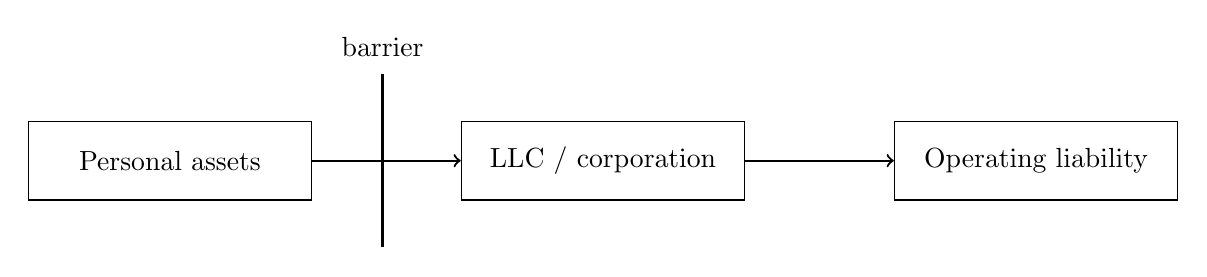
\begin{tikzpicture}[x=1cm,y=1cm]
\node[draw, rectangle, minimum width=3.6cm, minimum height=1cm] (p) at (0,0) {Personal assets};
\node[draw, rectangle, minimum width=3.6cm, minimum height=1cm] (e) at (5.5,0) {LLC / corporation};
\node[draw, rectangle, minimum width=3.6cm, minimum height=1cm] (l) at (11,0) {Operating liability};
\draw[->, thick] (p) -- (e);
\draw[->, thick] (e) -- (l);
\draw[thick] (2.7,-1.1) -- (2.7,1.1);
\node at (2.7,1.45) {barrier};
\end{tikzpicture}
\caption{A transcript-backed liability shield. The interview provides commercial function, not formal legal doctrine: the operating entity is supposed to keep business shocks from directly reaching the private balance sheet.}
\end{figure}

The host then recaps the lesson in sponsor-shaped language, saying that many entrepreneurs build the business and skip the foundation. We should keep that beat because it is part of the lecture's rhythm, but not allow it to dominate the section. Its role is pedagogical: the guest states the risk; the host translates it into a general rule.

\section{Beverly Hills II: Dealmaking, Patents, and the Propagation of Opportunity}

The second Beverly Hills interview shifts us from defensive structure to offensive opportunity. Jeffrey Phillips gives several doctrines at once. He says that dealmakers make a lot of money, that the ``smartest'' man is the man closest to God, that he owns gaming patents, that his company is worth \$1.2 billion, and that when he states a target publicly the world begins sending him introductions.

\subsection{Question \& Answer}

\paragraph{Question.}
How does a \$48 million commission happen?

\paragraph{Answer.}
In this lecture's answer, not by scholastic brilliance alone, but by position. One overhears a need, knows another party, connects the two, and stands at the point where information becomes transaction.

The numerical content is explicit enough for a worked example.

\paragraph{Worked example: the casino transaction.}
\begin{align}
D_{\mathrm{casino}} &\approx \$450\times 10^6, \\
C_{\mathrm{commission}} &\approx \$48\times 10^6, \\
\alpha_{\mathrm{commission}}
&=
\frac{C_{\mathrm{commission}}}{D_{\mathrm{casino}}}
\approx
\frac{48}{450}
\approx
0.107.
\end{align}

So the implied take is about \(10.7\%\). The interview never states that percentage. It gives only the raw amounts. But the arithmetic is worth doing because it shows us how large the economics of brokerage can become when the intermediary sits at the right junction.

The same speaker gives a valuation marker and a life-stage marker:

\begin{equation}
V_{\mathrm{gaming\,company}} \approx \$1.2\times 10^9,
\qquad
a_{\mathrm{millionaire}} \approx 27,
\qquad
a_{\mathrm{current}} \approx 58.
\end{equation}

Again, the lecture does not use these numbers as audited proof. It uses them to build authority for the mechanisms that follow.

The patent claim is also concrete. He says he owns the patents to the blackjack bonus-round structures, and when players use them he gets paid. Because the interview gives no royalty schedule, the strongest safe formalization is only proportional:

\begin{equation}
R_t \propto Q_t,
\end{equation}

where \(Q_t\) is play volume and \(R_t\) is the revenue stream attached to the patented mechanism. The whole point is that ownership of the rule can out-earn labor inside the rule.

A further motivational beat in this section should not be lost. When asked for the greatest advice he received, Jeffrey says it came from a doctor in Las Vegas while he was trying to raise money for his first television show: stop investing in other things and invest in yourself. That sentence matters because it joins faith to agency. The lecture is not presenting belief as passivity. It is presenting belief as permission to allocate capital, attention, and creative energy toward oneself.

This helps explain the more mystical line about declaring targets and watching the universe open. In practical form, the mechanism is simple enough to write schematically:

\begin{equation}
T_{\mathrm{declared}} \to N(T) \to I_{\mathrm{intro}} \to D_{\mathrm{deal}}.
\end{equation}

The claim is not deterministic. It is sociological. Public intention changes who knows what you want; once more people know, the odds of a relevant introduction rise.

\begin{figure}[h]
\centering
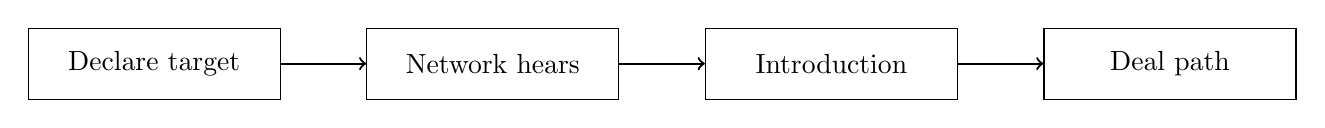
\begin{tikzpicture}[x=1cm,y=1cm]
\node[draw, rectangle, minimum width=3.2cm, minimum height=0.9cm] (t) at (0,0) {Declare target};
\node[draw, rectangle, minimum width=3.2cm, minimum height=0.9cm] (n) at (4.3,0) {Network hears};
\node[draw, rectangle, minimum width=3.2cm, minimum height=0.9cm] (i) at (8.6,0) {Introduction};
\node[draw, rectangle, minimum width=3.2cm, minimum height=0.9cm] (d) at (12.9,0) {Deal path};
\draw[->, thick] (t) -- (n);
\draw[->, thick] (n) -- (i);
\draw[->, thick] (i) -- (d);
\end{tikzpicture}
\caption{The lecture's opportunity-propagation mechanism, reconstructed from the transcript. Declared intention becomes network visibility, network visibility becomes contact, and contact becomes deal possibility.}
\end{figure}

The section closes with two additional beats that are easy to miss if we rush. First, Jeffrey says he has gone broke and could make it back again. Second, he explains that confidence by appeal to belief in God, belief in himself, and what he calls a creative mind. The lecture is therefore quietly building a composite view of entrepreneurial power: spiritual conviction, commercial position, and the capacity to improvise are not presented as alternatives but as reinforcements.

\section{Las Vegas: Dana White's Risk Window and Product Vision}

Only after these two Beverly Hills voices does the lecture go to Las Vegas. The host's travel, the arrival at the UFC Performance Institute, the walk-through, and the ``full circle moment'' should remain visible in the notes because they are part of the transition logic. Dana White is not supposed to drop in as a theorem. He is entered through threshold, admiration, and place.

The interview begins with a very compressed self-description: ``I sell fights for a living.'' That line does in one sentence what the whole opening sought to do. It converts a vague aura of success into a brutal commercial noun and verb: there is a product, and he sells it.

Dana then goes backward. Before the UFC he was working as a bellman in Boston. The important phrase is not that he was ``meant for more,'' which the interviewer offers, but that the job was simply not him. This distinction matters. Destiny is too theatrical; mismatch is more exact. He did not dislike work. He disliked that work.

From there he gives the lecture's rule about timing risk. When one is \(19\), \(20\), \(21\), even into one's thirties, and before children or heavier responsibilities arrive, one should take the risk because one can still go back if it fails. The form of the argument is practical, not romantic. A reversible risk is not the same thing as no risk, but it is not yet trapped risk either.

\subsection{Question \& Answer}

\paragraph{Question.}
What did he see in the UFC that others did not?

\paragraph{Answer.}
He and his partners loved the storylines, thought the fighting was more exciting than boxing, and believed they could keep what they loved in boxing while removing what they hated.

The compact symbolic summary is therefore

\begin{equation}
\text{UFC product}
\approx
\text{boxing}_{\mathrm{loved}}
-
\text{boxing}_{\mathrm{hated}}
+
\text{MMA intensity/storylines}.
\end{equation}

This notation is editorial, not historical. Its value is that it keeps the lecture from becoming vague. Dana White's disruption story is not pure novelty. It is redesign. He does not say, we invented combat. He says, we took a form people already loved, stripped away parts they hated, and made the whole package more exciting.

This is why the later advice to entrepreneurs has real substance. ``Break the rules'' in this interview does not mean indulge chaos. It means inspect any rule that has survived merely because no one has challenged it in a very long time. A century-old convention is not yet a law of nature.

\section{Repeated Proof, Competition, and Loyalty}

Now the lecture makes one of its strongest turns. Having explained vision, it refuses triumphalism. The interviewer asks whether there was ever a time when it felt as though the UFC might collapse. Dana answers, yes, one goes through that all the time. Even now, after a huge new deal, the proving does not end.

\subsection{Question \& Answer}

\paragraph{Question.}
What does it mean to keep proving yourself after you have already won?

\paragraph{Answer.}
It means that scale enlarges the burden rather than abolishing it. Success increases the size of the platform, but it does not remove recurrence. January arrives, and the proof has to be made again.

The largest explicit number in the Dana section appears here:

\begin{equation}
D_{\mathrm{Paramount}} = \$7.7\times 10^9.
\end{equation}

But the lecture does not linger on the number for its own sake. It immediately pairs it with the phrase ``fresh slate.'' That pairing is the point. The Italy ritual each Christmas---the temporary withdrawal, the days on the boat, the growing impatience to attack the next year---is a recovery mechanism inside a repeated-proof cycle.

Competition then enters not as a separate topic but as the emotional tone of recurrence. Dana says he loves competition. He says that people who called him a bully are often people who tried to compete and lost. The business world is phrased as a fight, which means there will be winners and losers.

Yet the lecture immediately complicates that warlike stance by pivoting to loyalty. If one's word is everything, then aggression must be balanced by obligation. This becomes concrete in the COVID discussion. Dana says he was not going to lay off employees simply because revenue stopped flowing. He presents the company as a battleship: either all go down together or not at all.

Then comes a beautiful piece of entrepreneurial mechanics. The usual route was blocked. There was a product. There was a venue problem. There was a transmission problem. There were broadcast partners who still needed the content. So the system had to be redrawn.

\begin{figure}[h]
\centering
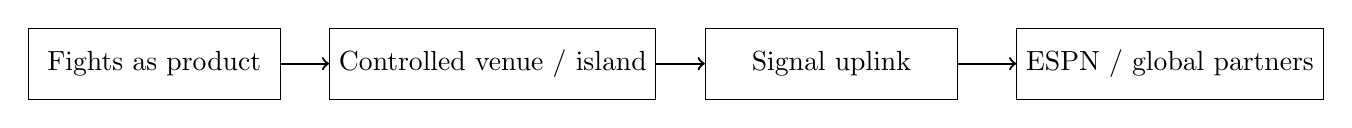
\begin{tikzpicture}[x=1cm,y=1cm]
\node[draw, rectangle, minimum width=3.2cm, minimum height=0.9cm] (p) at (0,0) {Fights as product};
\node[draw, rectangle, minimum width=3.2cm, minimum height=0.9cm] (v) at (4.3,0) {Controlled venue / island};
\node[draw, rectangle, minimum width=3.2cm, minimum height=0.9cm] (s) at (8.6,0) {Signal uplink};
\node[draw, rectangle, minimum width=3.2cm, minimum height=0.9cm] (n) at (12.9,0) {ESPN / global partners};
\draw[->, thick] (p) -- (v);
\draw[->, thick] (v) -- (s);
\draw[->, thick] (s) -- (n);
\end{tikzpicture}
\caption{The COVID workaround as a transcript-backed distribution diagram. The lecture's operational claim is that if the ordinary path is blocked, we redesign the route rather than abandoning the product.}
\end{figure}

The famous line ``don't tell me something can't be done'' sits exactly here, and now its meaning is sharper. It is not generic optimism. It is logistics with refusal added to it. If the system can be decomposed into product, venue, transmission, and audience, then each obstruction can be attacked as a design problem.

\section{Consistency and the Daily Update Rule}

The final movement compresses the entire interview into one recurrence. When asked what the most successful people have in common, Dana answers: consistency. He then adds the necessary condition underneath it: to have consistency, one must also have drive.

The generational exchange that follows should not be flattened into mere complaint. Dana says his generation would run over the younger one, but then he immediately tells the interviewer that it is easier than ever to stand out. Why? Because the visible winners in the new economy are not accidental. They are grinding, touring, reinvesting their own money, believing in themselves, and working far more than outsiders think. In other words, the lecture returns to its recurring theme: glamour outside, machinery beneath.

The interviewer then asks for the greatest advice of a lifetime, and Dana's answer does not become a sentimental parable. It becomes a statement of wiring: when you build something great, everybody is coming for a piece of it, and if you do not jump out of bed ready for war, you will not last. That rhetoric is severe, but the lecture is not content to end on severity. It keeps going until it reaches something closer to a rule.

Near the end Dana gives the sentence he has lived by since childhood: do not place limits on what can be done, and every day try to be better than the day before. Here the lecture finally condenses all of its earlier machinery into a single update condition.

\subsection{Question \& Answer}

\paragraph{Question.}
How do we beat yesterday?

\paragraph{Answer.}
Not by waiting for a dramatic break in fortune, and not by confusing intensity with direction, but by imposing an order relation on successive states.

\begin{equation}
X_{t+1} > X_t.
\end{equation}

The variable \(X_t\) is deliberately broad because the interview itself broadens it. It may refer to business execution, physical condition, relationships, or disciplined conduct. The lecture's point is precisely that these domains are not isolated. The same recurrence is supposed to govern all of them.

\begin{definition}
Let \(X_t\) denote the state of a chosen domain on day \(t\): business, fitness, relationships, or disciplined character. The lecture's closing demand is to prefer trajectories for which \(X_{t+1} > X_t\) whenever comparison is meaningful.
\end{definition}

At this stage we can also understand why the coda about weakness and jealousy lands where it does. The chapter has spent twenty minutes reducing business mythology to repeated, structured effort. ``Beat yesterday'' is therefore not a motivational slogan placed over emptiness. It is the final abstraction of the whole lecture. If the state does not improve, then the theater of confidence has outrun its mechanism.

\section{Summary}

The lecture begins with scale and ends with recurrence. Between those endpoints it builds a chain: work matters, asymmetry matters, allocation matters, structure matters, intermediary position matters, rights matter, faith and self-investment matter, product redesign matters, loyalty matters, and success never cancels the next proof.

It also preserves a strong narrative rhythm. We are not allowed to arrive at Dana White too quickly. Beverly Hills comes first because the lecture wants to hand us a vocabulary before it hands us the larger case. Then Las Vegas arrives as a threshold, and only after that threshold does the main doctrine unfold: the old job was not the right life, the risk had to be taken before responsibility calcified, the product had to be redesigned rather than merely inherited, and the company had to keep proving itself even after it was enormous.

If we compress the chapter to its final operational form, the sequence is this. Build before you boast. Protect before you scale. Own the rule, the right, or the junction rather than mere activity. Redesign the stale incumbent form. When the route is blocked, redraw the route. And then, after all the stories and all the scale claims, keep only the recurrence that survives the whole lecture:

\begin{equation}
X_{t+1} > X_t.
\end{equation}

That is the interview's hardest-won piece of mathematics. It is minimal, but it is not thin. It is the rule by which the lecture converts wealth, entrepreneurship, and character into something we can test one day at a time.